\section{Computational Structure}\label{chpt:fmm:sec:computational_structure}

- The data flow is shown in Figure \ref{fig:chpt:fmm:data_flow} for all the operators for a uniform FMM in two dimensions with two levels taken in the hierarchical tree.

As expressed in the preceding section on may have a pessimistic view on obtaining performance for a given FMM implementation as it relies on:

- nonlinear hierarchical data structure - resulting in non-linear data access patterns, illsuited to the data movement requirements of modern hardwares.

- A double recursion through a hierarchical data structure.

- A number of `operators' that define linear transformations between data associated with each box at each level during the hierarchical recursion.

- A critical operator, M2L, which necessarily relies on data non-local to a given box.

- The long range interactions captured by the recursive tree loop and the M2L operator leading to an O(N) algorithm, are also features which mean that practical implementations on modern computers where flops are no longer a good proxy for the runtime complexity of a software.

- Algorithm implementations must instead focus heavily on data operations such as transfer, synchrnoisations, and attempt to heavily utilise the cache available to us in modern CPUs/GPUs to minimise data transfer, even at the cost of extra flops - as extra flops on locally cached data represent a modest increase in the runtime/energy usage.

However, there are also many positives

- Expensive operations involving particle data at the leaf level can be efficiently parallelised due to natural expression via SIMT/SIMD approaches.

- The M2M/L2L operators offer clear opportunities for data re-use over siblings as they are operating between parent/child boxes.

- These operators can therefore be expressed very high arithmetic intensity. Which we define as the ratio of \textit{useful flops per memory access}.

- Although at first glance the M2L and the recursive application of operators seem to be barriers to achieving high arithmetic intensity overall for the FMM, it's clear that symmetry arguments can be used to batch together applications of M2L operators across multiple boxes if the kernels defining the interaction exhibit translational invariance.
- Furthermore, the tree is considered level-wise in a highly consistent fashion across all levels. And therefore offers significant opportunities for linear data layout for all required data per tree level.

- Therefore, although the FMM at first glance appears to be an algorithm with significant data access issues and cache problems due to its recursive structure and reliance on a hierarchical data structure, it can be seen when unrolled that it is in principle expressable using linear data structures where all operators have opportunities for high-arithmetic intensity formulations.
- as we show in figure ... where we sketch the data flow operation in Figure \ref{fig:chpt:fmm:data_flow} as an unrolled FMM loop, with linear data access.

\begin{figure}[h]
    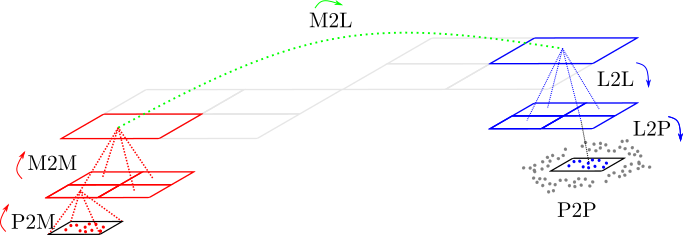
\includegraphics[width=\textwidth]{fmm_data_flow.png}
    \caption{Data flow for the evaluation of the potentials due to a given set of (red) source particles in the far field of a given set of (blue) target particles, in two dimensions for clarity with a uniform tree of depth two. The source particles in the near field of the target box are shown in grey.}
    \label{fig:chpt:fmm:data_flow}
\end{figure}

- Many past works have alluded to this feature of the FMM, though it is rarely expressed as such explicitly in the literature.

- Early examples include the works of Chandramowlishwaram and co-workers, who develop performance models characterising the kiFMM on various hardwares, and acknowledge the trade-off between the M2L and P2P as the key characteristic for FMM performance, and controlled by the tree depth.
- Deeper trees, synonymous with fewer particles per leaf node, and therefore smaller $U$-lists for P2P, but with more M2L.
- Shallower trees, synonymous with larger P2P and fewer M2L.

- Since then many works have focussed on expressing the data dependencies explicitly, and exposing them to special runtimes. - Proponent of task based runtime systems, as not restricted to specific algorithmic ordering of tasks removes artificial syncs, expose more native concurrency, and shorten critical path. The latter tends to restrict operations to a specific order. DAG-based dynamic runtime engines can remove artifactual synchronizations in the form of subroutine boundaries, remove artifactual orderings in the form of pre-scheduled loops, expose the native concurrency, and shorten the critical path. StarPU, Charm++ and Legion being popular runtimes.

- However as we can see there are remarkably few intra-level synchrnoisations required for the FMM, meaning that the overhead of a runtime system in comparison to ordinary multithreading based appraoches

- The principal drawback of losing this control is that though NUMA aware approaches do exist, it is significantly hardware to control data locality, which i§s critical for performance on modern architectures.

- Furthermore, most critically, the two most expensive operations of the FMM, the P2P and M2L operators, \textit{have no data dependencies} Meaning that there is amply opportunity to develop fully asynchronous implementations of these two operations, and given the optimal SIMD/SIMT structure of the P2P operation the obvious choice of operator to deploy to GPU in a heterogenous implementation.


